
%% for embedding info into PDF metadata via the hyperref package
%\def\doctitle{}
%\def\docauthor{}

\documentclass[10pt]{article}
\usepackage[latin1]{inputenc}
\usepackage[english]{babel}
\usepackage[none]{hyphenat}
\sloppy  %% this actually gives better linebreaks, minimising overhanging text
\usepackage[T1]{fontenc}
%\usepackage{url}
\usepackage[includefoot,includehead,left=2cm,right=2cm,top=1cm,bottom=2cm]{geometry}
\usepackage[usenames,dvipsnames]{color}  % see http://en.wikibooks.org/wiki/LaTeX/Colors
%\usepackage[pdfborder={0 0 0},colorlinks=true,urlcolor=blue,linkcolor=blue,citecolor=blue,bookmarks=true,pdftitle={\doctitle},pdfauthor={\docauthor}]{hyperref}
\usepackage[pdfborder={0 0 0},colorlinks=true,urlcolor=blue,linkcolor=blue,citecolor=blue,bookmarks=true]{hyperref}
\usepackage[numbers]{natbib}
\usepackage{graphicx}
%\usepackage[draft]{minted}
\usepackage{minted}
\usepackage{authblk}
\usepackage{amsmath}
\usepackage{amsthm}
\usepackage{bm}
\usepackage{booktabs}      % for \toprule in tables
\usepackage{multirow}      % for table multirow
\usepackage{tcolorbox}   % colorbox in minted
\usepackage{times}
%\usepackage{palatino}     % changes the default sans serif font
\usepackage{inconsolata}   % changes the default typewriter font
\usepackage{adjustbox}
\usepackage{threeparttable}
\usepackage{parcolumns}
\usepackage{amsfonts}
\usepackage{nicefrac}
\usepackage{microtype}
\usepackage{tabularx}
\usepackage{array}
\usepackage{wasysym}

% disable ligatures such as "fi" being joined into one symbol
\usepackage{microtype}
\DisableLigatures[f]{encoding = *, family = * }

\renewcommand{\baselinestretch}{1.1}\small\normalsize

\newcolumntype{R}[2]{%
  >{\adjustbox{angle=#1,lap=\width-(#2)}\bgroup}%
  l%
  <{\egroup}%
}
\newcommand*\rot{\multicolumn{1}{R{30}{2.0em}}}

\def\TODO#1{{\color{red}{\bf [TODO:} {{#1}}{\bf ]}}}

\begin{document}

\begin{center}

%{\Large {\tt ensmallen}: accelerating mathematical optimization via template metaprogramming}
{\Large\bf The ensmallen library for efficient mathematical optimization}
%% CS: simpler title to avoid frightening people away by the scary words "template" and "metaprogramming"

\vspace{1.5ex}
{Ryan Curtin~{$^1$}, Marcus Edel~{$^2$}, Conrad Sanderson~{$^{3,4}$}, ...}
\vspace{1.5ex}

\begin{tabular}{l}
$^1$~RelationalAI, Atlanta, USA\\
$^2$~Free University of Berlin, Germany\\
$^3$~Data61~/~CSIRO, Australia\\
$^4$~Griffith University, Australia
\end{tabular}

\end{center}


\section*{Abstract}

%\begin{small}
This report provides an introduction to the {\tt ensmallen} numerical optimization library,
as well as a deep dive into the technical details of how it works.
The library provides a fast and flexible C++ framework
for mathematical optimization of arbitrary user-supplied functions.
A large set of pre-built optimizers is provided,
including many variants of Stochastic Gradient Descent and Quasi-Newton optimizers.
Several types of objective functions are supported, including differentiable,
separable, constrained, and categorical objective functions.
Implementation of a new optimizer requires only one method,
while a new objective function requires typically only one or two C++ methods.
Through internal use of C++ template metaprogramming, {\tt ensmallen} provides support for arbitrary
user-supplied callbacks and automatic inference of unsupplied methods without
any runtime overhead.
Empirical comparisons show that {\tt ensmallen}
outperforms other optimization frameworks (such as Julia and SciPy), sometimes
by large margins.  The library is available at \url{https://ensmallen.org}
and is distributed under the permissive BSD license.
%\end{small}

% and is ready for use in productions environments.  
%% Commented out, as it's a subjective statement;
%% whether it's "ready" for a specific "production environment"
%% is up to the user.
%% Stating the BSD license is already a big hint that
%% people can do whatever they want with it,
%% and that there are no guarantees of fitness
%% for a particular purpose.
%% https://tldrlegal.com/license/bsd-3-clause-license-(revised)#fulltext




\vspace{4ex}
\hrule


\section{Introduction}
\label{sec:introduction}

The problem of mathematical optimization is fundamental in the computational
sciences.  In short, this problem is expressed as
%
\begin{equation}
\operatornamewithlimits{argmin}_x f(x)
\end{equation}

\noindent
where $f(x)$ is a given objective function and $x$ is typically a vector or matrix.
The ubiquity of this problem gives rise to the proliferation of mathematical
optimization toolkits, such as SciPy~\cite{2019arXiv190710121V},
opt++~\cite{meza1994opt++},
OR-Tools~\cite{ortools}, CVXOPT~\cite{vandenberghe2010cvxopt},
NLopt~\cite{johnson2014nlopt}, Ceres~\cite{ceres-solver},
%% {\tt fminsearch()} in MATLAB~\cite{matlab_fminsearch},
and RBFOpt~\cite{costa2018rbfopt}.
Furthermore, in the field of machine learning, many
deep learning frameworks have integrated optimization
components.  Examples include Theano~\cite{2016arXiv160502688},
TensorFlow~\cite{tensorflow2015-whitepaper}, PyTorch~\cite{NEURIPS2019_9015},
and Caffe~\cite{jia2014caffe}.

Mathematical optimization is generally quite computationally intensive.
For instance, the training of deep neural networks is dominated by
the optimization of the model parameters on the
data~\cite{krizhevsky2012imagenet, lauzon2012introduction}.  Similarly,
other popular machine learning algorithms such as logistic regression are also
expressed as and dominated by an optimization process~\cite{zhang2004solving,
manogaran2018health}.  Computational bottlenecks occur even in fields as
wide-ranging as rocket landing guidance systems~\cite{dueri2016customized},
motivating the development and implementation of specialized solvers.

The necessity for both efficient and specializable function optimization motivated us
to implement the {\tt ensmallen} library, originally as part of the {\tt mlpack}
machine learning library~\cite{mlpack2018}.
The {\tt ensmallen} library provides a large {set of pre-built optimizers} for optimizing
{user-defined objective functions} in C++;
at the time of writing, 46 optimizers are available.  
The external interface to the optimizers is intuitive and matches the ease of use of popular
optimization toolkits mentioned above.

However, unlike many of the existing optimization toolkits,
{\tt ensmallen} explicitly supports numerous function types:
arbitrary, differentiable, separable, categorical, constrained, and semidefinite.
Furthermore, custom behavior during optimization can be easily specified via {\it callbacks}.
Lastly, the underlying framework facilitates the implementation of new optimization techniques,
which can be contributed upstream and incorporated into the library.
Table~\ref{tab:comparison} contrasts the functionality supported
by {\tt ensmallen} and other optimization toolkits.

This paper is a revised and expanded description of our initial overview
of {\tt ensmallen}~\cite{ensmallen2018}. 
It also provides a deep dive into the internals
of how the library works, which can be a useful resource for anyone looking
to contribute to the library or get involved with its development.

%% TODO: this will need to be refactored once the document is refactored
% In this paper, we describe the details of the template metaprogramming
% techniques and how we are able to simultaneously produce efficient code and a
% clean user interface.

\TODO{update}
The paper is continued as follows.
We introduce the functionality and interface for {\tt ensmallen} in Section~\ref{sec:api}.
Section~\ref{sec:templated_optimize} shows how {\tt ensmallen} can optimize objective functions
$f(x)$ for various types of $x$ without any extra runtime overhead.
Section~\ref{sec:automatic} discusses the details of how {\tt ensmallen} is able
to automatically generate methods not provided by the user.
Section~\ref{sec:callbacks} describes {\tt ensmallen}'s callbacks.
We demonstrate the empirical efficiency of {\tt ensmallen} in
Section~\ref{sec:experiments} and conclude in Section~\ref{sec:conclusion}.


\begin{table}[!t]
\centering
    \begin{tabular}{@{} cl*{9}c @{}}
%  \begin{tabular}{ccccccc}
        & & \multicolumn{7}{c}{} \\[0.6ex]
            % If there is any coherent framework at all, this is true.
        & & \rot{unified framework}
            % If there is any support for constrained optimization, this is
            % true.
          & \rot{constraints}
            % If the optimization framework can do mini-batch, this is true.
          & \rot{separable functions / batches}
            % If I can implement any arbitrary function to be optimized, this is
            % true.
          & \rot{arbitrary functions}
            % If I can implement any new optimization technique to use, this is
            % true.
          & \rot{arbitrary optimizers}
            % If the framework could take advantage of when the gradient is
            % sparse, this is true.
          & \rot{sparse gradients}
            % If the framework can handle categorical/discrete variables for
            % optimization, this is true.
          & \rot{categorical}
            % If any type can be optimized, this is true.mention
          & \rot{arbitrary types}
            % If callback support is available.
          & \rot{callbacks} \\
        \cmidrule[1pt]{2-11}
        % It might be reasonable to say mlpack categorical support is only
        % partial, but I am not sure exactly where we draw the line.
        & \texttt{ensmallen}            & \CIRCLE & \CIRCLE & \CIRCLE & \CIRCLE & \CIRCLE & \CIRCLE & \CIRCLE & \CIRCLE & \CIRCLE\\
        % The Shogun toolbox has a fairly nice framework, but it doesn't support
        % sparse gradients or categorical features.  It also does not appear to
        % support constraints, arbitrary types, or callbacks.
        & Shogun \cite{sonnenburg2010shogun}             & \CIRCLE & - & \CIRCLE
& \CIRCLE & \CIRCLE & - & - & - & - \\
        % VW doesn't appear to have any framework whatsoever and the code is
        % awful, but it does support batches and categorical features.
        & Vowpal Wabbit \cite{Langford2007VW}      & - & - & \CIRCLE  & - & - & - &
\CIRCLE & - & - \\
        % TensorFlow has a few optimizers, but they are all SGD-related.  You
        % can write most objectives easily (but some very hard), and categorical
        % support might be possible but would not be easy.
        & TensorFlow \cite{tensorflow2015-whitepaper}        & \CIRCLE & -  & \CIRCLE  & \LEFTcircle & - &
\LEFTcircle & - & \LEFTcircle & - \\
        % Caffe has a nice framework, but it's only for SGD-related optimizers.
        % I think I could write a new one, but it is not the easiest thing in
        % the world.
        & Caffe \cite{jia2014caffe}           & \CIRCLE & -  & \CIRCLE & \LEFTcircle & \LEFTcircle
& - & - & \LEFTcircle & \CIRCLE \\
        % Keras is restricted to neural networks and SGD-like optimizers.  I
        % don't know that it is possible to easily write a new optimizer.
        & Keras \cite{chollet2015keras}            & \CIRCLE & -  & \CIRCLE & \LEFTcircle & \LEFTcircle
& - & - & \LEFTcircle & \CIRCLE \\
        % sklearn has a few optimizer frameworks, but they are all in different
        % places and have somewhat different support.
        & scikit-learn \cite{pedregosa2011scikit}       & \LEFTcircle & - & \LEFTcircle  & \LEFTcircle & -
& - & - & \LEFTcircle & - \\
        % scipy has some nice optimizer framework but it does not support
        % batches or some of the more complex functionality.  And you can't
        % write your own.
        & SciPy \cite{jones2014scipy}             & \CIRCLE & \CIRCLE  & -  &
\CIRCLE & - & - & - & \LEFTcircle & \CIRCLE \\
        % MATLAB is very similar to scipy.
        & MATLAB \cite{matlab_fminsearch}            & \CIRCLE & \CIRCLE & - &
\CIRCLE & - & - & - & \LEFTcircle & - \\
        % Optim.jl isn't the only Julia package for optimization, but it's the
        % one we compare against.
        & Julia (\texttt{Optim.jl}) \cite{mogensen2018optim}         &
\CIRCLE & - & - & \CIRCLE & - & - & - & \CIRCLE & - \\
        \cmidrule[1pt]{2-11}
    \end{tabular}
\caption{
Feature comparison: \CIRCLE~= provides feature,
\LEFTcircle~= partially provides feature, -~= does not provide feature.
{\it unified framework} indicates if there is a form of generic/unified
optimization framework; {\it constraints} and {\it separable functions /
batches} indicate support for constrained functions and separable functions;
{\it arbitrary functions} means arbitrary objective functions are easily
implemented; {\it arbitrary optimizers} means arbitrary optimizers are easily
implemented; {\it sparse gradient} indicates that the framework can natively
take advantage of sparse gradients; {\it categorical} refers to if support
for categorical features exists; {\it arbitrary types} mean that arbitrary types
can be used for the parameters $x$;
{\it callbacks} indicates that user-implementable callback support is available.
%\TODO{may want to add a comparison with PyTorch, as that's getting popular these days}
}
\label{tab:comparison}
\vspace{1ex}
\hrule
\end{table}


\section{API overview and examples}
\label{sec:api}

{\tt ensmallen} provides a {\bf set of optimizers} for optimizing {\bf
user-defined objective functions}.  These optimizers are generic and flexible,
meaning that they can support a wide range of use cases and applications.  A
primary differentiator from other toolkits is that this flexibility is provided
via template metaprogramming, which means that it comes at no runtime cost.
In addition to allowing users to easily define and optimize their own objective
functions, {\tt ensmallen} also makes it easy to implement new optimizers, which
can then be contributed back upstream and incorporated into the library.

Overall, our primary goal is to provide an easy-to-use and efficient library
that can solve the problem $\operatorname{argmin}_x f(x)$ for any function
$f(x)$ that takes a vector or matrix input $x$.  In most cases, $f(x)$ will have
some structure; one simple example might be that $f(x)$ is differentiable.
Therefore, the abstractions that we have built for {\tt ensmallen} can
optionally take advantage of this structure.  In the example of a differentiable
function $f(x)$, the user can provide an implementation of the gradient $f'(x)$,
which in turn allows a first-order optimizer to be used.  This generally leads
to significant, order-of-magnitude speedups.

To codify these structures, {\tt ensmallen}'s optimizers are made to accept
different types of objective functions.  These classes of objectives functions
are listed below.

\begin{itemize}
\item {\bf Arbitrary functions} ({\tt \small ArbitraryFunctionType}).  No
assumptions can be made on an arbitrary function $f(x)$ and only the objective
$f(x)$ can be computed for a given $x$.

\item {\bf Differentiable functions} ({\tt \small DifferentiableFunctionType}).
A differentiable function $f(x)$ is an arbitrary function whose gradient $f'(x)$
can be computed for a given $x$, in addition to the objective.

\item {\bf Partially differentiable functions} ({\tt \small
PartiallyDifferentiableFunctionType}).  A partially differentiable function
$f(x)$ is a differentiable function with the additional property that the
gradient $f'(x)$ can be decomposed along some basis $j$ such that $f_j'(x)$ is
sparse.  Often, this is used for coordinate descent algorithms (i.e., $f'(x)$
can be decomposed into $f_{x1}'(x)$, $f_{x2}'(x)$, etc.).

\item {\bf Arbitrary separable functions} ({\tt \small
ArbitrarySeparableFunctionType}).  An arbitrary separable function is an
arbitrary function $f(x)$ that can be decomposed into the sum of several
objective functions:

\begin{equation}
f(x) = \sum_i f_i(x).
\end{equation}

\item {\bf Differentiable separable functions} ({\tt \small
DifferentiableSeparableFunctionType}).  A differentiable separable function is a
separable arbitrary function $f(x)$ where the individual gradients $f_i'(x)$ are
also computable.

\item {\bf Categorical functions} ({\tt \small CategoricalFunctionType}).  A
categorical function type is an arbitrary function $f(x)$ where some (or all)
dimensions of $x$ take discrete values from a set.

\item {\bf Constrained functions} ({\tt \small ConstrainedFunctionType}).  A
constrained function $f(x)$ is a differentiable function\footnote{In general, it
is not a requirement that a constrained function is differentiable.  But we
require it here, as all {\tt ensmallen}'s current optimizers for constrained
functions require a gradient to be available.} subject to constraints of the
form $c_i(x)$; when the constraints are satisfied, $c_i(x) = 0\; \forall \; i$.
Minimizing $f(x)$ then means minimizing $f(x) + \sum_i c_i(x)$.
  \subitem {\bf Semidefinite programs} (SDPs).  {\tt ensmallen} has special
support to make optimizing semidefinite
programs~\cite{vandenberghe1996semidefinite} simple.
\end{itemize}

Details about how to implement and use each type of objective function can be
found on the {\tt ensmallen} website, at \url{https://ensmallen.org/docs.html}.

Using this straightforward abstraction framework, {\tt ensmallen} is able to
provide a wide range of optimizers:

\begin{itemize}
  \item {\bf For arbitrary functions.}  TODO

  \item {\bf For differentiable functions.}  TODO

  \item {\bf For partially differentiable functions.}  TODO

  \item {\bf For arbitrary separable functions.}  TODO

  \item {\bf For differentiable separable functions.}  TODO

  \item {\bf For categorical functions.}  TODO

  \item {\bf For constrained functions.}  TODO
\end{itemize}

Table \ref{table:comparison} compares the types of objective functions supported
by {\tt ensmallen} and other optimization toolkits.

The task of optimizing an objective function with {\tt ensmallen} is
straightforward.  The class of objective function (e.g., arbitrary, constrained,
differentiable, etc.) defines the implementation requirements.  For instance, if
a user wants to optimize some objective function $f(x)$ that is differentiable,
they merely need to provide an implementation of $f(x)$ and $f'(x)$ and then
they can immediately use one of {\tt ensmallen}'s optimizers for differentiable
functions.  That is, each objective function type has some minimal set of
methods that must be implemented.  Typically this is only between one and four
methods.

Note that not every type of objective function can be used with every type of
optimizer.  For instance, {\tt L\_BFGS} is a differentiable optimizer, and so it
cannot be used with any non-differentiable object function type (e.g. an
arbitrary function).  However, {\tt ensmallen} still allows as much flexibility
as possible via template metaprogramming:

\begin{enumerate}
  \item When an optimizer is used with a user-provided objective function,
template metaprogramming is used along with static assertions to provide
user-friendly error messages if any required methods are not detected.

  \item When possible, {\tt ensmallen} will automatically infer methods that are
not provided.  For instance, given a separable objective function where an
implementation of $f_i(x)$ is provided (as well as the number of such separable
objectives), an implementation of $f(x)$ can be inferred.  This is all done at
compile-time, and so there is no additional runtime overhead compared to a
handwritten implementation.
\end{enumerate}

To give an example, consider the example of linear regression, where we are
given a matrix of predictors $\bm X \in \mathcal{R}^{n \times d}$ and a vector
of responses $\bm y \in \mathcal{R}^n$.  Our task is to find the best linear
model $\bm \theta \in \mathcal{R}^d$; that is, we want to find $\bm \theta^* =
\operatorname{argmin} f(\bm \theta)$ for

\begin{equation}
f(\bm \theta) = \| \bm X \bm \theta - \bm y \|^2 = (\bm X \bm \theta - \bm y)^T
(\bm X \bm \theta - \bm y).
\label{eqn:obj_lr}
\end{equation}

From this we can easily derive the gradient $f'(\bm \theta)$:

\begin{equation}
f'(\bm \theta) = 2 \bm X^T (\bm X \bm \theta - \bm y).
\label{eqn:grad_lr}
\end{equation}

If we want to use {\tt ensmallen} to find $\bm \theta^*$ using a differentiable
optimizer, we simply need to provide implementations of $f(\bm \theta)$ and
$f'(\bm \theta)$ according to the signatures required by the {\tt
DifferentiableFunctionType} of objective function.  For a differentiable
function, only two methods are necessary: {\tt Evaluate()} and {\tt Gradient()}.
The introductory discussion here does not go into the full details of the
different signatures required for each objective function; for that, see the
{\tt ensmallen} documentation: \url{https://ensmallen.org/docs.html}.

Returning to our linear regression example, we could easily use {\tt ensmallen}'s
L-BFGS implementation to find $\bm \theta^*$; we just need to provide an
implementation of $f(\bm \theta)$ and $f'(\bm \theta)$ (as L-BFGS requires a
differentiable objective function).  Below is an example implementation.

\begin{minted}{c++}
class LinearRegressionFunction
{
 public:
  LinearRegressionFunction(const arma::mat& X, const arma::vec& y) : X(X), y(y)
  { }

  double Evaluate(const arma::mat& coordinates)
  {
    return (X * coordinates - y).t() * (X * coordinates - y);
  }

  void Gradient(const arma::mat& coordinates, arma::mat& gradient)
  {
    gradient = 2 * X.t() * (X * coordinates - y);
  }

  // Note that ensmallen gives us the option of only implementing *one* function
  // EvaluateWithGradient() instead, which would be more efficient in this case
  // since it can share computation between Evaluate() and Gradient()!
  //
  // (We use both Evaluate() and Gradient() here for simplicity of exposition.)

 private:
  const arma::mat& X;
  const arma::vec& y;
};
\end{minted}

In this example, we hold {\tt \small X} and {\tt \small y} as members of the
class, and {\tt \small coordinates} is used to represent $\bm \theta$.  Via the
use of Armadillo~\cite{TODO}, the linear algebra expressions to implement the
objective function and gradient are readable in a way that closely matches
Equations~\ref{eqn:obj_lr} and \ref{eqn:grad_lr}.  With {\tt \small
LinearRegressionFunction} implemented, we can easily find $\bm \theta^*$ with
the following code that uses {\tt ensmallen}'s L-BFGS optimizer:

\begin{minted}{c++}
// We assume that "X" and "y" are given.
LinearRegressionFunction f(X, y);

L_BFGS optimizer; // Create the optimizer with all default parameters.

// The theta_best matrix will hold the best model that we find after we call
// Optimize(); for now, we set it to the initial point (uniform random values).
arma::mat theta_best(X.n_rows, 1, arma::fill:randu);

optimizer.Optimize(f, theta_best);
\end{minted}

However, it's possible to do more than optimize a model that's stored as an {\tt
\small arma::mat} (dense matrix).  {\tt ensmallen} supports:

\begin{itemize}
  \item Use of types other than {\tt \small arma::mat} when calling {\tt \small
Optimize()}.  This can include integer-valued matrices, sparse matrices, or any
type whose implementation matches the Armadillo API.

  \item Callbacks, which can specify custom behavior during the optimization.
Examples include printing the loss function value at each iteration, or
terminating when a time budget is used up, or other custom user-supplied
functionality.

  \item Inference of functions not supplied by the user.  One example is that
for a differentiable function, a user might supply a {\bf joint} implementation
of the {\tt Gradient()} and {\tt Evaluate()} methods, instead of implementing
them separately.  {\tt ensmallen} can automatically infer variants of {\tt
Gradient()} and {\tt Evaluate()} when needed.
\end{itemize}

Each of the following sections will discuss how we are able to achieve the
functionality above---with no runtime overhead.

\section{Type-Agnostic Optimization}
\label{sec:templated_optimize}

% We can start by expanding on the linear regression function example to point
% out that we may want different types.

\begin{figure}[b!]
\hrule
\vspace{1ex}
\begin{minted}{c++}
class GradientDescent
{
  template<typename FunctionType, typename MatType, typename GradType = MatType>
  typename MatType::elem_type Optimize(FunctionType& function, MatType& coordinates)
  {
    // The step size is hardcoded to 0.01, and the number of iterations is 1000.
    for (size_t i = 0; i < 1000; ++i)
    {
      GradType gradient;
      function.Gradient(coordinates, gradient);

      // Take the step.
      coordinates -= 0.01 * gradient;
    }

    // Compute and return the final objective.
    return function.Evaluate(coordinates);
  }
};
\end{minted}
\hrule
\vspace*{-0.5em}
\caption{Example implementation of a simple gradient descent optimizer.
For the sake of brevity, functionality such as the ability to configure the parameters has
been deliberately omitted.
The actual {\tt GradientDescent} optimizer {\tt ensmallen} provides more functionality.
}

\label{fig:gd}
\end{figure}

In the example shown in Section~\ref{sec:linreg_example},
where we introduced the class {\tt LinearRegressionFunction},
the matrix and vector objects are hardcoded as {\tt arma::mat} and {\tt arma::vec}.
These objects hold elements with the C++ type {\tt double},
representing double precision floating point.
However, in many applications it can be very important to specify a different
underlying element type.  For instance, in the field of machine learning, neural
networks have been shown to be effective with low-precision floating point
representations for weights~\cite{vanhoucke2011improving}.
%% low-precision integers~\cite{courbariaux2015training},
%% or even single bits~\cite{courbariaux2015binaryconnect}.
Furthermore, many optimization problems have parameters
that are best represented as sparse data~\cite{van2011sparse, recht2011hogwild},
which is represented in Armadillo as the {\tt sp\_mat} class~\cite{sanderson2018user, mca24030070}.
Even alternate representations such as data held on the GPU can be quite
important: the use of GPUs can often result in significant
speedups~\cite{oh2004gpu, athanasopoulos2011gpu}.

In order to handle this diverse set of needs, {\tt ensmallen} has been built in
such a way that any underlying storage type can be used to represent the
coordinates to be optimized---so long as it matches the Armadillo API.
This means that the Bandicoot GPU matrix library\footnote{\url{https://gitlab.com/conradsnicta/bandicoot-code}}
can be used as a drop-in replacement once it is stable.

Consider the simplified gradient descent optimizer shown in Figure~\ref{fig:gd}.
The use of the template types {\tt FunctionType}, {\tt MatType}, and {\tt
GradType} means that at compilation time, the correct types are substituted in
for {\tt FunctionType}, {\tt MatType}, and {\tt GradType} (which by default is
set to be the same as {\tt MatType} in this code).  So long as each type has all
the methods that are used inside of {\tt Optimize()}, there will be no
compilation problems.  Templates are a technique for code generation; in this
case, that means the code generated will be exactly the same as if {\tt
Optimize()} was written with the types specified in those template parameters.
This means that there is no additional runtime overhead when a different {\tt
MatType} is used.

% TODO: this to a later details section?

However, there is one important drawback of C++ that we must work around when
providing support for any {\tt MatType}, and that is the issue of compiler
errors.  The compiler may fail to substitute a given {\tt MatType} into the
code above for {\tt GradientDescent::Optimize()}; a typical reason might be that
some needed method of {\tt MatType} or {\tt FunctionType} is not available.
For example, the given {\tt MatType} does not have an {\tt operator\*()} method.
When this happens, most current C++ compilers will emit a very long list
of error messages, with all relevant information about the attempted
template instantions.
This onslaught of error messages can be confusing and discouraging to users.
{\tt ensmallen} avoids this issue via the use of C++ compile-time static
assertions ({\tt static\_assert()}).
Users who are interested in the details of how these assertions work should
refer to Section~\ref{sec:templated_optimize_details}.

Note that users who would like to continue despite these {\tt static\_assert()}
checks failing may simply define the macro {\tt ENS\_DISABLE\_TYPE\_CHECKS} in
their code before the line {\tt \#include <ensmallen.hpp>}.


% TODO: this section name isn't particularly great...
\section{Automatic function generation}
\label{sec:automatic}

In this section the goals are to:

\begin{itemize}
  \item Introduce {\tt EvaluateWithGradient()} and the motivation for that
(logistic regression is a nice example).

  \item Point out that a user doesn't need to implement {\bf both} {\tt
Evaluate()} and {\tt EvaluateWithGradient()} but instead that we can
automatically infer one from the other {\it at compile time}.

  \item Discuss the general design of the template metaprogramming system that
makes this work.
\end{itemize}

\section{Callbacks}
\label{sec:callbacks}

Many optimizers offer the ability to modify the optimization process. Examples
include changing the step size, adding custom constraints when they are violated
by the current solution, or providing custom heuristics to find and investigate
feasible solutions.

In the past this functionality was limited to solver-specific interfaces [], in
contrast, ensmallen provides, optimizer independent callbacks to allow guidance
of the optimization process and to monitor the behavior of optimization. In
particular, ensmallen's callbacks allow code to be executed regularly during an
optimization session. To use callbacks, either for optimization, tuning or
logging, a user can pass arbitrary callbacks to any optimizer in the Optimize()
function. Figure~\ref{fig:example_prog_callbacks} contains a simple C++ program which briefly demonstrates usage of the callback functionaility.

\begin{figure}[H]
\centering
\hrule
\vspace{1ex}
\begin{adjustbox}{minipage=\columnwidth,scale={0.90}{0.85}}
\begin{minted}{c++}
RosenbrockFunction f;
arma::mat coordinates = f.GetInitialPoint();

MomentumSGD optimizer(0.01, 32, 100000, 1e-5, true, MomentumUpdate(0.5));
optimizer.Optimize(f, coordinates, EarlyStopAtMinLoss(), ProgressBar());
\end{minted}
\end{adjustbox}
\vspace{1ex}
\hrule
\caption
  {
  A simple C++ program to demonstrate usage of the callback functionality using pre-defined callbacks: \texttt{EarlyStopAtMinLoss()} and \texttt{ProgressBar}.
  }
\label{fig:example_prog_callbacks}
\end{figure}

Given the pre-defined callbacks {\tt EarlyStopAtMinLoss()} and {\tt
ProgressBar()} the code snippet above shows not only how the Momentum-SGD
optimizer can be used to find the best coordinates but also how the callbacks
can be used to control and overview the optimization process by calling the
callbacks at different stages of the optimization process.\newline

There are eight types of optimization callback routines that are regularly
called during the optimization process (depending on the function type).
Table~\ref{tab:callback_list} lists the available types.

\begin{table}[H]
\centering
\small
\begin{tabular}{lll}
\toprule
{\bf Function} & {\bf Description} & {\bf Function type} \\
\hline
\texttt{BeginOptimization}   & Called at the beginning of the optimization process  & all \\
\texttt{EndOptimization}     & Called at the end of the optimization process        & all \\
\texttt{Evaluate}            & Called after any call to {\it Evaluate()}            & Arbitrary, Differentiable, Partially differentiable,  \\
                             &                                                      & Arbitrary separable, Differentiable separable \\
\texttt{EvaluateConstraint}  & Called after any call to {\it EvaluateConstraint()}  & Constrained \\
\texttt{Gradient}            & Called after any call to {\it Gradient()}            & Differentiable, Partially differentiable \\
                             &                                                      & Differentiable separable \\
\texttt{GradientConstraint}  & Called after any call to {\it GradientConstraint()}  & Constrained \\
\texttt{BeginEpoch}          & Called at the beginning of a pass over the data      & Differentiable separable \\
\texttt{EndEpoch}            & Called at the end of a pass over the data            & Differentiable separable \\

\bottomrule
\end{tabular}
\vspace{0.5ex}
\caption
  {
  Available callback routines, with brief descriptions.
  Optional additional arguments have been omitted for brevity.
  See {\href{http://www.ensmallen.org/docs.html}{\mbox{\tt http://www.ensmallen.org/docs.html}}} for more detailed documentation.
  }
\label{tab:callback_list}
\end{table}

Callbacks are executed in the order that they are specified, by default
subsequent callbacks are discared if a callback terminates the optimization
process under circumstances defined by the application. To terminate the
optimiation process via callbacks, each callback routine can return an boolean,
true to continue, or false to indicate that the optimization process should be
terminated.

\begin{figure}[H]
\centering
\hrule
\vspace{1ex}
\begin{adjustbox}{minipage=\columnwidth,scale={0.90}{0.85}}
\begin{minted}{c++}
class CustomCallback
{
  template<typename OptimizerType, typename FunctionType, typename MatType>
  bool Evaluate(OptimizerType& optimizer,
                FunctionType& function,
                const MatType& coordinates,
                const double objective)
  {
    return true;  // Continue the optimization process.
  }
};
\end{minted}
\end{adjustbox}
\vspace{1ex}
\hrule
\caption
  {
  Control the optimization process via the return value of the callback routine.
  }
\label{fig:example_prog_callbacks}
\end{figure}

If a callback requires additional parameters beyond what is passed through
the predefined arguments, a user is encouraged to manully instantiate an object
with them, and pass the object or access optimizer specific parameter via the
optimizer interface. ensmallen does not modify or dereference the object, so it
is safe to use for this purpose.

\begin{figure}[H]
\centering
\hrule
\vspace{1ex}
\begin{adjustbox}{minipage=\columnwidth,scale={0.90}{0.85}}
\begin{minted}{c++}
struct CustomCallback
{
  CustomCallback(double rIn) : p(rIn) {}

  template<typename OptimizerType, typename FunctionType, typename MatType>
    void StepTaken(OptimizerType& optimizer,
                   FunctionType& function,
                   MatType& coordinates)
    {
      optimizer.StepSize() *= r;
    }

  double r;
};

RosenbrockFunction f;
arma::mat coordinates = f.GetInitialPoint();

Adam opt;
CustomCallback cb(0.9);
opt.Optimize(f, coordinates, cb);
\end{minted}
\end{adjustbox}
\vspace{1ex}
\hrule
\caption
  {
  A simple C++ program of adding additional parameter to a Callback and accessing optimizer specific parameter.
  }
\label{fig:example_prog_callbacks_parameter}
\end{figure}

In this example~\ref{fig:example_prog_callbacks_parameter}, we pass an
instatiated custom callback that takes an additional step-size decay parameter
as input, in addition, inside the {\tt StepTake()} callback we use the optimizer
interface ({\tt StepSize()}) to update the step size.

To demonstrate the advantages of the template-based optimization mechanism, we
performed a set of experiments~\ref{fig:callback_compilter_opt}, that compared
the machine code of an optimizer with callback support and without. In all
cases, a modern C++ compiler [] optimized away the non-used code, the resultant
machine code appears as if the never existed in the first place.

\begin{figure}[H]
\centering
\hrule
\hrule
\vspace{0.5ex}
\begin{minipage}{0.45\textwidth}
\begin{minted}[fontsize=\footnotesize,stripnl=false]{c++}
struct Optimizer
{
  template<typename FT>
  void Optimize(FT& f, arma::mat& p)
  {
    f.Evaluate(p);
  }
};

void main()
{
  RosenbrockFunction rf;
  arma::mat parameters = rf.GetInitialPoint();
  Optimizer opt;
  opt.Optimize(rf, parameters);
}

\end{minted}
\end{minipage}
%
\hfill
\vline
\vline
\hfill
%
\begin{minipage}{0.45\textwidth}
\begin{minted}[escapeinside=||,fontsize=\footnotesize]{c++}
struct Optimizer
{
  template<typename FT, |\colorbox{yellow}{typename... CallbackType}|>
  void Optimize(FT& f, arma::mat& p, CallbackType&&... c)
  {
    |\colorbox{yellow}{Callback::BeginOptimization(*this, f, p, c...);}|
    f.Evaluate(iterate);
  }
};
void main()
{
  RosenbrockFunction rf;
  arma::mat parameters = rf.GetInitialPoint();
  Optimizer opt;
  opt.Optimize(rf, parameters);
}
\end{minted}
\end{minipage}
\vspace{0.5ex}
\hrule
\hrule
\caption
  {
  Left panel: A C++ program that mimics the ensmallen optimizer interface
  without any callback functionality. Right panel: A corresponding C++ program
  using an empty callback routine that is automatically optimized out. Both
  programs produce the exact same machine code, resulting in no performance
  penalty if no callbacks are used.
  }
\label{fig:callback_compilter_opt}
\end{figure}

For the sake of brevity we omit the expressions for the {\tt BeginOptimization}
method \footnote{Interested readers can find that code in {\tt
ensmallen\_bits/callbacks/callbacks.hpp}.}. The function depend heavily on
SFINAE techniques for method detection; {\tt HasBeginOptimization} will evaluate
to {\tt true} if {\tt CallbackType} has {\tt BeginOptimization()} and {\tt
false} otherwise.

Using the boolean template variable, we can then use template specialization to
control whether {\tt BeginOptimization} returns a boolean, void to control the
optimization process or if the callback ends in an empty function
call.











A custom callback is a powerful tool to customize the behavior of a function
during the optimization process. Examples include {\tt StoreBestCoordinates<>()}
where the model is automatically saved during the optimization process or {\tt
EarlyStoppingAtMinLoss()}  which stops the optimization process when the minimum
of loss has been reached.

\begin{figure}[H]
\centering
\hrule
\vspace{1ex}
\begin{adjustbox}{minipage=\columnwidth,scale={0.90}{0.85}}
\begin{minted}{c++}
class EarlyStoppingAtMinLoss
{
 public:
  // Set up the early stopping at min loss class, which keeps track of the
  // minimum loss.
  EarlyStop() : bestObjective(std::numeric_limits<double>::max()) { }

  // Callback function called at the end of a pass over the data, which provides
  // the current objective. We are only interested in the objective and ignore
  // the rest.
  template<typename OptimizerType, typename FunctionType, typename MatType>
  void EndEpoch(OptimizerType&, FunctionType&, const MatType&, const size_t,
                const double objective)
  {
    // Check if the given objective is lower as the previous objective.
    if (objective < bestObjective)
    {
      bestObjective = objective; // Update the local objective.
    }
    else
    {
      return true; // Stop the optimization process.
    }

    return false; // Do not stop the optimization process.
  }

  double bestObjective;
};
\end{minted}


\begin{minted}{c++}
// We assume that "X" and "y" are given.
LinearRegressionFunction f(X, y);

L_BFGS optimizer; // Create the optimizer with all default parameters.

// The theta_best matrix will hold the best model that we find after we call
// Optimize(); for now, we set it to the initial point (uniform random values).
arma::mat theta_best(X.n_rows, 1, arma::fill:randu);

// Optimize the given function and provide a callback (EarlyStoppingAtMinLoss)
// that is called at the end of an epoch.
optimizer.Optimize(f, theta_best, EarlyStoppingAtMinLoss());
\end{minted}
\end{adjustbox}
\vspace{1ex}
\hrule
\caption
  {
  A simple C++ program that demonstrates the implementation of a custom callback function.
  }
\label{fig:example_prog_callbacks_parameter}
\end{figure}

Please see a complete list and description of ensmallens's callback functions in
the callback documentation. In addition, we recommend closely reviewing the
examples provided in
\url{include/ensmallen_bits/callbacks}
which provide examples of how to use most of these callback functions.

\section{Experiments}
\label{sec:experiments}

To demonstrate the benefits of the metaprogramming based code optimizations
that {\tt ensmallen} can exploit, we compare the performance of {\tt ensmallen}
with several other optimization frameworks, including some that use automatic
differentiation.

\begin{figure}[b!]
\hrule
\vspace{1ex}
\begin{minted}{c++}
#include <ensmallen.hpp>

struct RosenbrockFunction
{
  template<typename MatType>
  static typename MatType::elem_type Evaluate(const MatType& x) const
  {
    return 100 * std::pow(x[1] - std::pow(x[0], 2), 2) + std::pow(1 - x[0], 2);
  }
};

int main()
{
  // We use Armadillo's timing functionality to print how long it takes to optimize.
  arma::wall_clock clock;

  RosenbrockFunction rf;
  ens::ExponentialSchedule sched;
  // A tolerance of 0.0 means the optimization will run for the maximum number of iterations.
  ens::SA<> s(sched, 100000, 10000, 1000, 100, 0.0);

  // Get the initial point of the optimization.
  arma::mat parameters = rf.GetInitialPoint();

  // Run the optimization and time it.
  clock.tic();
  s.Optimize(rf, parameters);
  const double time = clock.toc();
  std::cout << time << std::endl << "Result (optimal 1, 1): " << parameters.t();
}
\end{minted}
\hrule
\vspace*{-0.5em}
\caption{Code to use {\tt ensmallen} to optimize the Rosenbrock function using
100k iterations of simulated annealing.}
\label{fig:rosenbrock_run}
\end{figure}

\subsection{Simple optimizations and overhead}

For our first experiment, we aim to capture the overhead involved in different
optimization toolkits.  In order to do this, we consider the simple and popular
Rosenbrock function~\cite{Rosenbrock1960}:

\begin{equation}
f([x_1, x_2]) = 100 (x_2 - x_1^2)^2 + (1 - x_1^2).
\end{equation}

This objective function is useful for this task because the computational effort
involved in computing $f(\cdot)$ is trivial.  Therefore, if we hold the number
of iterations of each toolkit constant, then this will help us understand the
different overhead costs of each toolkit.  For the optimizer, we use simulated
annealing~\cite{kirkpatrick1983optimization}, a gradient-free optimizer.
Simulated annealing will call the objective function numerous times; for each
simulation we limit the optimizer to 100k objective evaluations.

The code used to run this simulation for {\tt ensmallen} (including the
implementation of the Rosenbrock function) is given in
Figure~\ref{fig:rosenbrock_run}.  Note that the {\tt RosenbrockFunction} is
actually implemented in {\tt ensmallen}'s source code, in the directory {\tt
include/ensmallen\_bits/problems/}.

\begin{table}[t]
\begin{center}
\begin{tabular}{lcccc}
\toprule
 & {\tt ensmallen} & {\tt scipy} & {\tt Optim.jl} & {\tt samin} \\
\midrule
default & {\bf 0.004s} & 1.069s & 0.021s & 3.173s \\
tuned & & 0.574s & & 3.122s \\
\bottomrule
\end{tabular}
\end{center}
\vspace*{-0.5em}
\caption{Runtimes for $100000$ iterations of simulated annealing with various
frameworks on the simple Rosenbrock function.  Julia code runs do not count
compilation time.  The {\it tuned} row indicates that the code was manually
modified for speed.}
\label{tab:rosenbrock_results}
\end{table}

% TODO: code snippet comparison for each language?

We compare four frameworks for this task:

\begin{itemize}
  \item[{\bf (i)}] {\tt ensmallen},
  \item[{\bf (ii)}] {\tt scipy.optimize.anneal} from SciPy 0.14.1~\cite{jones2014scipy},
  \item[{\bf (iii)}] simulated annealing implementation in {\tt Optim.jl} with Julia 1.0.1~\cite{mogensen2018optim},
  \item[{\bf (iv)}] {\tt samin} in the {\tt optim} package for Octave~\cite{octave}.
\end{itemize}

While another option here might be {\tt simulannealbnd()}
in the Global Optimization Toolkit for MATLAB,
no license was available.
We ran our code on a MacBook Pro i7 2018 with 16GB RAM running macOS 10.14 with clang 1000.10.44.2, Julia version 1.0.1, Python 2.7.15, and Octave 4.4.1.

Our initial implementation for each toolkit, corresponding to the line
``default'' in Table~\ref{tab:rosenbrock_results}, was as simple of an
implementation as possible and included no tuning.  This reflects how a typical
user might interact with a given framework.  Only Julia and {\tt ensmallen} are
compiled, and thus are able to avoid the function pointer dereference for
evaluating the Rosenbrock function and take advantage of inlining and related
optimizations.  The overhead of both {\tt scipy} and {\tt samin} are quite
large---{\tt ensmallen} is nearly three orders of magnitude faster for the same
task!

% TODO: keep removing \small from here

% Actually Octave's JIT is apparently some kind of prototype joke and it doesn't
% even compile anymore.  So MEX was the only way...
However, both Python and Octave have routes for acceleration,
such as Numba~\cite{lam2015numba}, MEX bindings and JIT compilation.
We hand-optimized the Rosenbrock implementation using Numba,
which required significant modification of the
underlying \texttt{\small anneal.anneal()} function.
These techniques did produce some speedup,
as shown in the second row of Table~\ref{tab:rosenbrock_results}.
For Octave, a MEX binding did not produce a noticeable difference.
We were unable to tune either \texttt{\small ensmallen} or \texttt{\small
Optim.jl} to get any speedup, suggesting that novice users will easily be able
to write efficient code in these cases.

\subsection{Large-scale linear regression problems}

\begin{table}[b!]
\centering
%\begin{adjustbox}{scale={0.90}{0.90}}
\begin{tabular}{lccccc}
\toprule
{\em algorithm} & $d$: 100, $n$: 1k & $d$: 100, $n$: 10k & $d$: 100, $n$:
100k & $d$: 1k, $n$: 100k \\
\midrule
\texttt{\small ensmallen}-1 & {\bf 0.001s} & {\bf 0.009s} & {\bf 0.154s} & {\bf 2.215s} \\
\texttt{\small ensmallen}-2 & 0.002s & 0.016s & 0.182s & 2.522s \\
% Dropped for space and awful performance
%\texttt{\small Calculus.jl} & 0.172s & 0.960s & 27.428s & 2535.507s \\
\texttt{\small Optim.jl} & 0.006s & 0.030s & 0.337s & 4.271s \\
\texttt{\small scipy} & 0.003s & 0.017s & 0.202s & 2.729s \\
\texttt{\small bfgsmin} & 0.071s & 0.859s & 23.220s & 2859.81s\\
% It's possible to tune ForwardDiff.jl a bit, but it doesn't give significant
% speedups to make it competitive and it really makes the code ugly.
\texttt{\small ForwardDiff.jl} & 0.497s & 1.159s & 4.996s & 603.106s \\
\texttt{\small autograd} & 0.007s & 0.026s & 0.210s & 2.673s \\
\bottomrule
\end{tabular}
%\end{adjustbox}
\vspace*{0.25ex}
\caption{
Runtimes for the linear regression function on various dataset sizes,
with $n$ indicating the number of samples,
and $d$ indicating the dimensionality of each sample.
All Julia runs do not count compilation time.}
\label{tab:lbfgs}
\end{table}

Next, we consider the linear regression example described in
Sec.~\ref{sec:linreg_example}.  For this task we use the first-order L-BFGS
optimizer~\cite{liu1989limited}, implemented in {\tt ensmallen} as the {\tt
L\_BFGS} class.  Using the same four packages, we implement
the linear regression objective and gradient.  Remembering that {\tt ensmallen}
allows us to share work across the objective function and gradient
implementations (Section~\ref{sec:automatic}), for {\tt ensmallen} we implement
a version with only {\tt EvaluateWithGradient()}, denoted as {\tt ensmallen-1}.
We also implement a version with both \texttt{\small Evaluate()} and
\texttt{\small Gradient()}: \texttt{\small ensmallen-2}.  We also use automatic
differentiation for Julia via the \texttt{\small
ForwardDiff.jl}~\cite{RevelsLubinPapamarkou2016} package and for Python via the
\texttt{\small Autograd}~\cite{maclaurin2015autograd} package.  For GNU Octave
we use the \texttt{\small bfgsmin()} function.

Results for various data sizes are shown in Table~\ref{tab:lbfgs}.  For each
implementation, L-BFGS was allowed to run for only $10$ iterations and never
converged in fewer iterations.  The datasets used for training are highly noisy random
data with a slight linear pattern. Note that the exact data is not relevant
for the experiments here, only its size.  Runtimes are reported as the
average across 10 runs.

The results indicate that \texttt{\small ensmallen} with \texttt{\small
EvaluateWithGradient()} is the fastest approach.
Furthermore, the use of \texttt{\small EvaluateWithGradient()} yields
non-negligible speedup over the \texttt{\small ensmallen-2} implementation with
both the objective and gradient implemented separately.  In addition, although
the automatic differentiation support makes it easier for users to write their
code (since they do not have to write an implementation of the gradient), we
observe that the output of automatic differentiators is not as efficient,
especially with \texttt{\small ForwardDiff.jl}.  We expect this effect to be
more pronounced with increasingly complex objective functions.

\subsection{Easy pluggability of different optimizers}

Lastly, we demonstrate the easy pluggability in \texttt{\small ensmallen}
for using various optimizers on the same task.
Using a version of {\tt LinearRegressionFunction} from
Section~\ref{sec:linreg_example} adapted for separable differentiable
optimizers, we run six optimizers with default parameters in just 8 lines of
code, as shown in Fig.~\ref{fig:learning_curve_code}.
Applying these optimizers to the \texttt{\small YearPredictionMSD}
dataset from the UCI repository~\cite{ucimlrepository}
yields the learning curves shown in Fig.~\ref{fig:learning_curve}(b).

\begin{figure}[b!]
\hrule
\vspace{1ex}
\begin{minted}{c++}
// X and y are data.
LinearRegressionFunction lrf(X, y);

using namespace ens;
StandardSGD<>().Optimize(lrf, sgdModel);
Adam().Optimize(lrf, adamModel);
AdaGrad().Optimize(lrf, adagradModel);
SMORMS3().Optimize(lrf, smorms3Model);
SPALeRASGD().Optimize(lrf, spaleraModel);
RMSProp().Optimize(lrf, rmspropModel);
\end{minted}
\hrule
\vspace*{-0.5em}
\caption{{\tt ensmallen} makes it easy to switch out optimizer types: 8
lines of code run 6 different optimizers on one problem.}
\label{fig:learning_curve_code}
\end{figure}

Any other optimizer for separable differentiable objective
functions can be dropped into place in the same manner; given {\tt ensmallen}'s
large number of available optimizers, this support could be used to easily
compare optimizers.  In fact, this is exactly done with the interactive
optimizer visualization tool found at \url{https://vis.ensmallen.org}.
Figure~\ref{fig:visualization} shows an example visualization from that page.

\begin{figure}[t!]
  \centering
  % 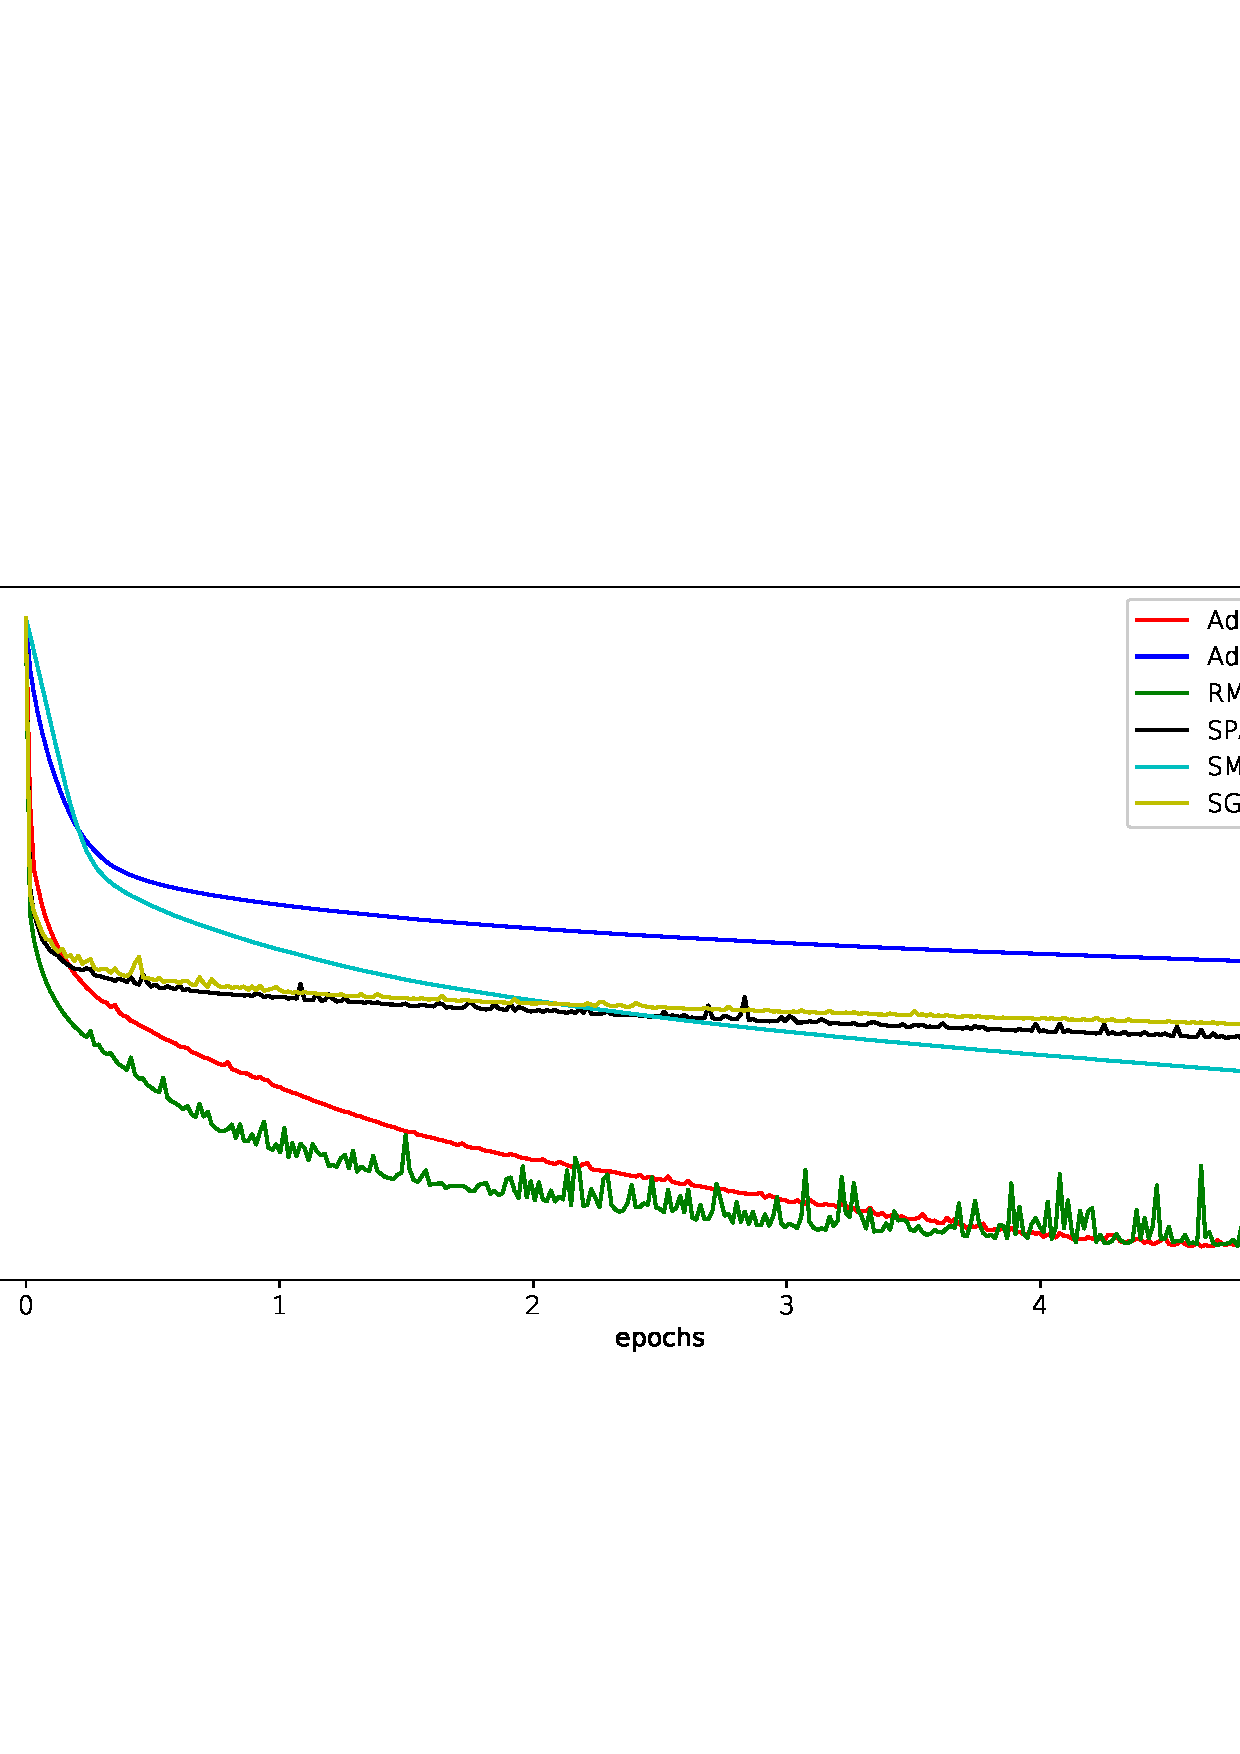
\includegraphics[width=\textwidth,height=0.45\textwidth]{experiments/learning_curves_crop.png}
  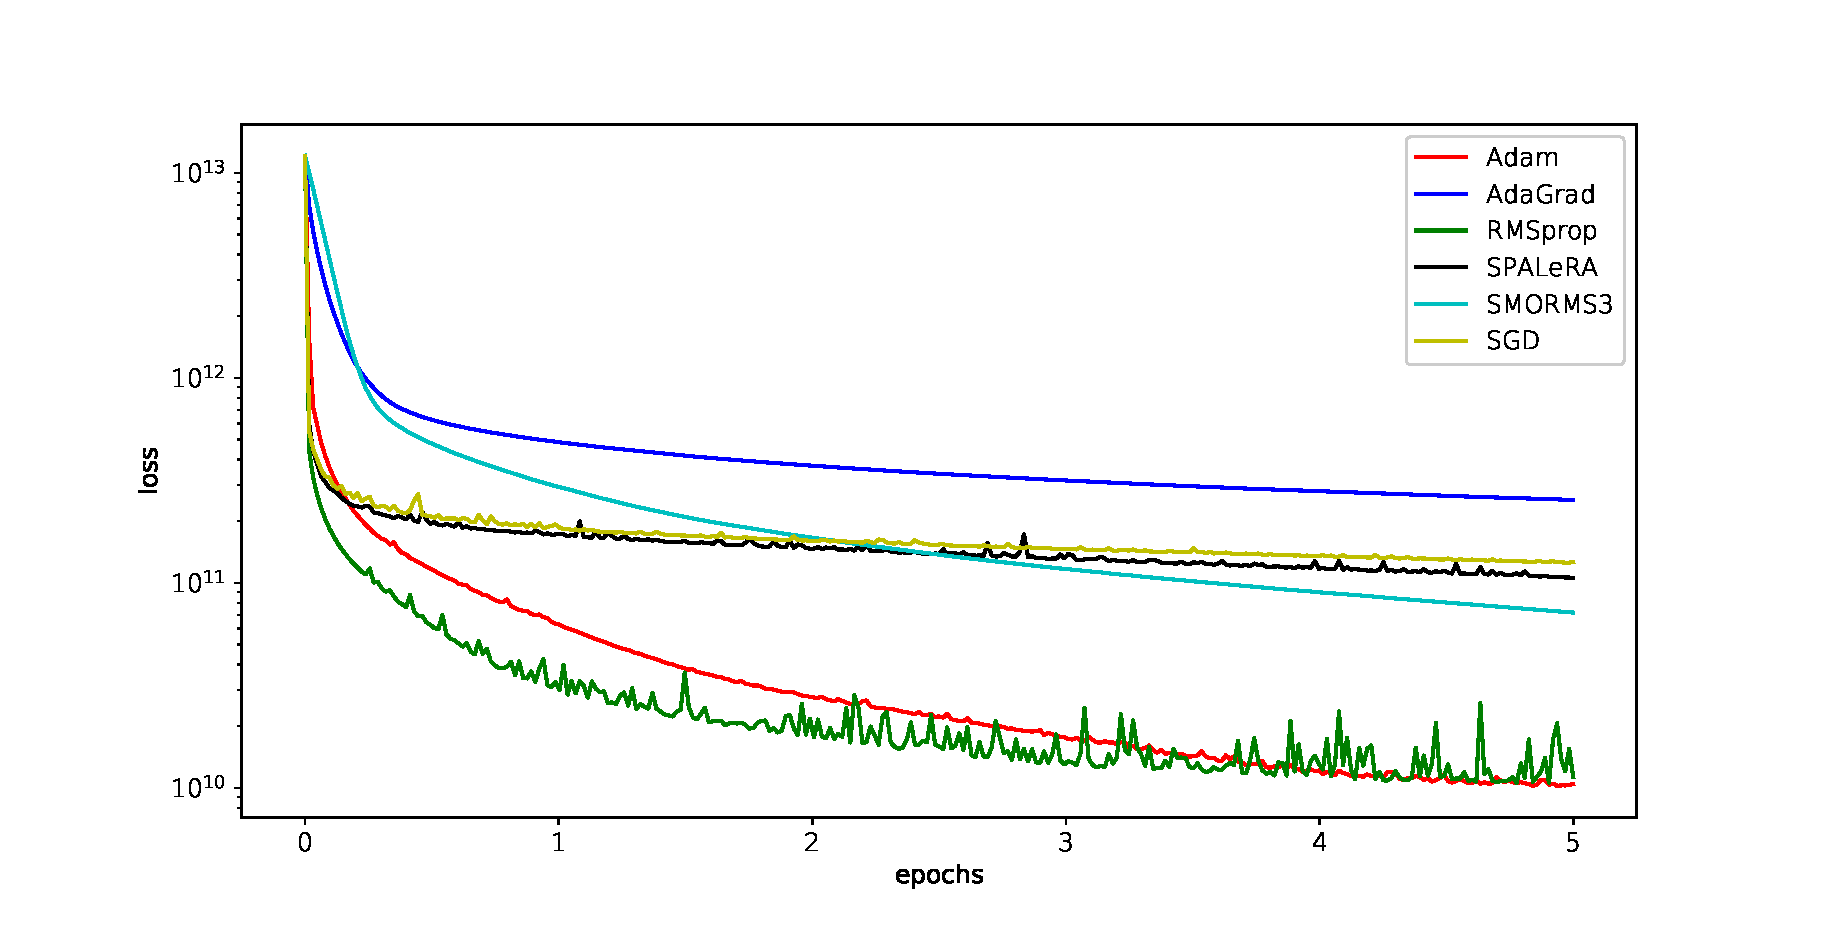
\includegraphics[width=\textwidth,height=0.5\textwidth]{experiments/learning_curves_crop.eps}
  %% CS: to remove the blank space around the plot:
  %% CS: epstool --copy --bbox input.eps output.eps
  \vspace*{-2.5em}
\caption{
Example usage of six {\tt ensmallen} optimizers to optimize a linear regression
function on the {\tt YearPredictionMSD} dataset~\cite{ucimlrepository} for 5
epochs of training.  The optimizers can be tuned for better performance.}
\label{fig:learning_curve}
\end{figure}

\begin{figure}[b!]
  \centering
  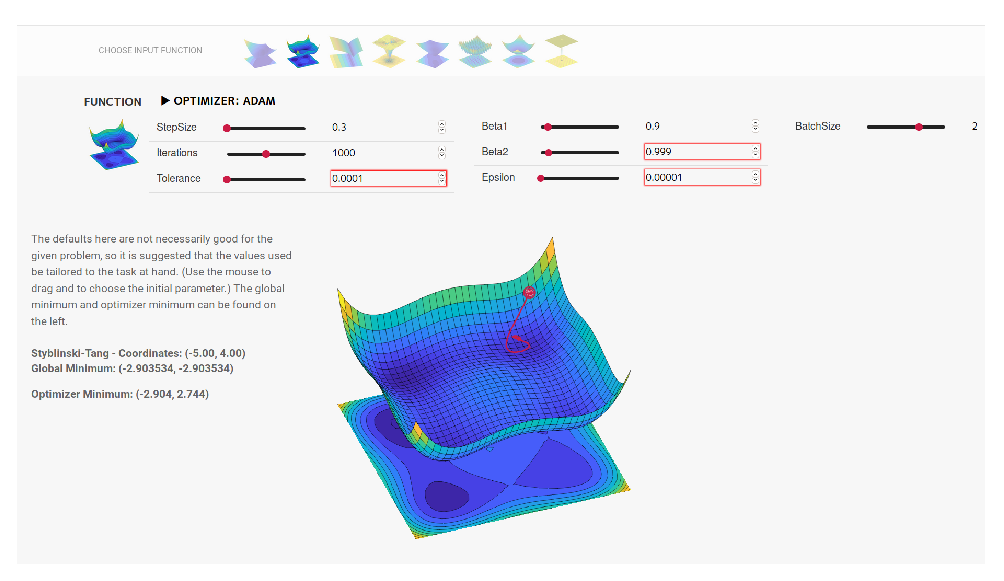
\includegraphics[width=\textwidth]{experiments/visualization.eps}
  \vspace*{-2em}
  \caption{Visualization of the Adam optimizer on the Styblinski-Tang objective
function; this is a screen capture from \url{https://vis.ensmallen.org}.}
  \label{fig:visualization}
\end{figure}


\section{Conclusion}
\label{sec:conclusion}

The goals of this section are just to conclude (we should write it last).



%\clearpage
% Could use \appendix here if we wanted, but I figured a \clearpage was enough.
\section{Static assertions to check matrix traits}
\label{sec:templated_optimize_details}

In Section~\ref{sec:templated_optimize}, we showed that {\tt ensmallen} uses
templates to allow arbitrary types to be used for the matrix type or gradient
type.  However, this requires some amount of special handling to ensure that the
user encounters a reasonable, comprehensible error message if the given matrix
or gradient type does not have the required methods.  Here, we discuss the
details of how we provide better error messages than the default onslaught of
compiler error messages via the use of {\tt static\_assert()}.

{\tt ensmallen} provides a few utility methods for checking traits of {\tt
MatType} and {\tt GradType} (for differentiable objective functions) inside of
an optimizer's {\tt Optimize()} method:

\begin{itemize}
  \item {\tt RequireFloatingPointType<MatType>()}: this requires that the
element type held by {\tt MatType} is either {\tt float} or {\tt double}.
This is generally needed by optimizers that use LAPACK or BLAS functionality.

  \item {\tt RequireSameInternalTypes<Mat1Type, Mat2Type>()}: this requires that
{\tt Mat1Type} and {\tt Mat2Type} use the same type to hold elements.  This can
be useful for differentiable optimizers, where we want to ensure, for example,
that a user can't pass a {\tt MatType} that holds {\tt int}s, but a {\tt GradType} that
holds {\tt unsigned int}s.

  \item {\tt RequireDenseFloatingPointType<MatType>()}: this requires that the
element type held by {\tt MatType} is either {\tt float} or {\tt double}, and
that the representation used for storage by {\tt MatType} is dense.
\end{itemize}

These methods would typically be called at the top of the implementation of an
optimizer's {\tt Optimize()} method.

At the time of writing, these are the only three checks that have
been needed, but it is easy to add more.  The implementation of these functions
is just a {\tt static\_assert()} that uses some underlying traits of the given
template parameters.  For example, Figure~\ref{fig:rsit} is the implementation
of {\tt RequireSameInternalTypes<...>()}.

\begin{figure}[t]
\hrule
\vspace{1ex}
\begin{minted}{c++}
/**
 * Require that the internal element type of the matrix type and gradient type
 * are the same.  A static_assert() will fail if not.
 */
template<typename MatType, typename GradType>
void RequireSameInternalTypes()
{
#ifndef ENS_DISABLE_TYPE_CHECKS
  static_assert(std::is_same<typename MatType::elem_type,
                             typename GradType::elem_type>::value,
      "The internal element types of the given MatType and GradType must be "
      "identical, or it is not known to work!  If you would like to try "
      "anyway, set the preprocessor macro ENS_DISABLE_TYPE_CHECKS before "
      "including ensmallen.hpp.  However, you get to pick up all the pieces if "
      "there is a failure!");
#endif
}
\end{minted}
\hrule
\vspace*{-0.5em}
\caption{Implementation of {\tt RequireSameInternalTypes()} from internal
{\tt ensmallen} code.
\TODO{This figure is probably not be necessary: it's trivial stuff. The
descriptions in the preceding bullet points are sufficient.  (Response from
Ryan: I agree, but I find that people new to mlpack are really scared of
actually *looking* at code and figuring out what it does.  This gives a direct
reference to code that's there, which is an entrypoint someone can use to then
learn more.  Anyway, it's in the back now, so maybe it's not a problem to leave
it in.  Let me know what you think.)}
}
\label{fig:rsit}
\end{figure}

\input{sections/automatic_details.tex}
\input{sections/callbacks_internals.tex}

\bibliographystyle{ieee}
\bibliography{refs}

\end{document}
